% !TeX program = xelatex
\documentclass[a4paper,10pt]{article}

% ============================================================================
% កញ្ចប់បណ្ណាល័យ (Packages) – តាមលំនាំ NGS Preah Krasang Scenario
% ============================================================================
\usepackage[a4paper, left=0.95cm, right=0.95cm, top=0.80cm, bottom=0.90cm, footskip=0.45cm]{geometry}
\usepackage{amsmath}
\usepackage{unicode-math}
\usepackage{fontspec}
\usepackage{array, longtable, multirow, colortbl}
\usepackage[table]{xcolor}
\usepackage{enumitem}
\usepackage{pifont}
\usepackage{fancyhdr}
\usepackage{tikz}
\usetikzlibrary{calc, arrows.meta, decorations.markings, babel}

% LaTeX 2025 + longtable v4.24 compatibility guard
\makeatletter
\let\@expl@@@mark@update@singlecol@structures@@\relax
\makeatother

% ============================================================================
% ការកំណត់ពុម្ពអក្សរ (Fonts Configuration) – តាមលំនាំស្ដង់ដារ ១០០%
% ============================================================================
% Cross-platform font path resolver (Windows local + Linux/Cloud repo fonts/)
\providecommand{\NGSFindFonts}{%
  \IfFileExists{C:/Windows/Fonts/cambria.ttc}{%
    \def\NGSSysPath{C:/Windows/Fonts/}%
    \def\NGSUserPath{C:/Users/KIT/AppData/Local/Microsoft/Windows/Fonts/}%
  }{%
    \IfFileExists{./fonts/KhmerOSsiemreap.ttf}{\def\NGSSysPath{./fonts/}\def\NGSUserPath{./fonts/}}{%
    \IfFileExists{../fonts/KhmerOSsiemreap.ttf}{\def\NGSSysPath{../fonts/}\def\NGSUserPath{../fonts/}}{%
    \IfFileExists{../../fonts/KhmerOSsiemreap.ttf}{\def\NGSSysPath{../../fonts/}\def\NGSUserPath{../../fonts/}}{%
    \IfFileExists{../../../fonts/KhmerOSsiemreap.ttf}{\def\NGSSysPath{../../../fonts/}\def\NGSUserPath{../../../fonts/}}{%
    \IfFileExists{../../../../fonts/KhmerOSsiemreap.ttf}{\def\NGSSysPath{../../../../fonts/}\def\NGSUserPath{../../../../fonts/}}{%
    \IfFileExists{../../../../../fonts/KhmerOSsiemreap.ttf}{\def\NGSSysPath{../../../../../fonts/}\def\NGSUserPath{../../../../../fonts/}}{%
    \IfFileExists{../../../../../../fonts/KhmerOSsiemreap.ttf}{\def\NGSSysPath{../../../../../../fonts/}\def\NGSUserPath{../../../../../../fonts/}}{%
      \def\NGSSysPath{../../../../../../../fonts/}\def\NGSUserPath{../../../../../../../fonts/}%
    }}}}}}}%
  }%
}
\NGSFindFonts

\setmathfont[
  Path={\NGSSysPath},
  FontIndex=1,
  Scale=1.02
]{cambria.ttc}

\defaultfontfeatures{Ligatures=TeX}

\setmainfont[
  Path={\NGSUserPath},
  Extension=.ttf,
  Script=Khmer,
  BoldFont={KhmerOSsiemreap},
  BoldFeatures={FakeBold=1.8},
  ItalicFont={KhmerOSsiemreap},
  ItalicFeatures={FakeSlant=0.25},
  BoldItalicFont={KhmerOSsiemreap},
  BoldItalicFeatures={FakeBold=1.8, FakeSlant=0.25}
]{KhmerOSsiemreap}

\newfontfamily\muol[
  Path={\NGSUserPath},
  Extension=.ttf,
  Script=Khmer
]{KhmerOSmuollight}

\newfontfamily\TimesEn[
  Path={\NGSSysPath},
  Extension=.ttf,
  Scale=1.00,
  BoldFont={timesbd},
  ItalicFont={timesi},
  BoldItalicFont={timesbi}
]{times}

\newfontfamily\NagaBold[
  Path={\NGSUserPath},
  Extension=.ttf
]{AKbalthom Naga Bold}

\newfontfamily\CalibriFont[
  Path={\NGSSysPath},
  Extension=.ttf
]{calibri}

\newfontfamily\CourierBullet[
  Path={\NGSSysPath},
  Extension=.ttf
]{cour}
\newcommand{\wcirc}{{\CourierBullet\fontsize{9pt}{10.5pt}\selectfont o}}

\XeTeXlinebreaklocale "km"
\XeTeXlinebreakskip = 0pt plus 1pt minus 0.1pt

% ============================================================================
% ការកំណត់ពណ៌ និងទម្រង់ទំព័រ (Colors & Page Style)
% ============================================================================
\definecolor{stepgray}{HTML}{D9D9D9}
\definecolor{headgray}{HTML}{F2F2F2}
\definecolor{boxgray}{HTML}{D9D9D9}
\definecolor{darkred}{HTML}{C00000}
\definecolor{red5e}{HTML}{FF0000}

\pagestyle{fancy}
\fancyhf{}
\renewcommand{\headrulewidth}{0pt}
\fancyfoot[R]{\CalibriFont\fontsize{10.5pt}{12pt}\selectfont\thepage}

\setlength{\parindent}{0pt}
\setlength{\parskip}{0pt}
\setlength{\tabcolsep}{3.5pt}
\renewcommand{\arraystretch}{1.04}

\newcolumntype{L}[1]{>{\raggedright\arraybackslash}p{#1}}

% ============================================================================
% ម៉ាក្រូជំនួយ (Helper Macros)
% ============================================================================
\newcommand{\en}[1]{{\TimesEn #1}}
\newcommand{\enbf}[1]{{\TimesEn\textbf{#1}}}
\newcommand{\unit}[1]{\,\text{\en{#1}}}
\newcommand{\fiveE}[1]{{\NagaBold\fontsize{8.8pt}{12pt}\selectfont\textcolor{red5e}{#1}}}
\newcommand{\timenote}[1]{\textcolor{darkred}{\textit{#1}}}
\newcommand{\cnum}[1]{{\fontsize{9.5pt}{11pt}\selectfont\ding{\numexpr181+#1\relax}}}
\newcommand{\tri}[1]{\ensuremath{\triangle #1}}
\newcommand{\ang}[1]{\ensuremath{\angle #1}}
\newcommand{\ditem}{\tikz[baseline=-0.5ex]\fill (0,0.38ex) -- (0.38ex,0) -- (0,-0.38ex) -- (-0.38ex,0) -- cycle;\hspace{0.25em}}

\tikzset{
  tk1/.style={postaction={decorate},decoration={markings,mark=at position 0.50 with {\draw[black, line width=0.8pt](0,-0.085)--(0,0.085);}}},
  tk2/.style={postaction={decorate},decoration={markings,
    mark=at position 0.45 with {\draw[black, line width=0.8pt](0,-0.085)--(0,0.085);},
    mark=at position 0.55 with {\draw[black, line width=0.8pt](0,-0.085)--(0,0.085);}}},
  tkslash/.style={postaction={decorate},decoration={markings,mark=at position 0.50 with {\draw[black, line width=0.8pt](-0.06,-0.07)--(0.06,0.07);}}}
}

% រូបផ្ទៀងផ្ទាត់រហ័ស (B&W Quick Reference: សម្រាយផ្ទាល់ ទំ.១៥៨ & ប្រតិបត្តិ ១០៨° ទំ.១៥៩)
\newcommand{\figScenarioRefINEQ}{%
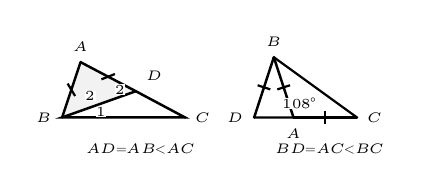
\begin{tikzpicture}[scale=0.52, every node/.style={font=\tiny, text=black}]
  % ឆ្វេង៖ សម្រាយផ្ទាល់ AD=AB<AC
  \begin{scope}[shift={(-2.30,0)}]
    \coordinate (B) at (-1.15,0);
    \coordinate (C) at (1.85,0);
    \coordinate (A) at (-0.70,1.35);
    \coordinate (D) at (0.65,0.64);
    \fill[gray!10] (A) -- (B) -- (D) -- cycle;
    \draw[black, line width=0.9pt, tkslash] (A) -- (B);
    \draw[black, line width=0.9pt, tkslash] (A) -- (D);
    \draw[black, line width=0.9pt] (D) -- (C) -- (B) -- (D);
    \fill[black] (A) circle (1.0pt) node[above=0.4pt] {$A$};
    \fill[black] (B) circle (1.0pt) node[left=0.4pt] {$B$};
    \fill[black] (C) circle (1.0pt) node[right=0.4pt] {$C$};
    \fill[black] (D) circle (1.0pt) node[above right=0.4pt] {$D$};
    \node[fill=white, inner sep=0.2pt] at (-0.46,0.52) {$2$};
    \node[fill=white, inner sep=0.2pt] at (-0.20,0.13) {$1$};
    \node[fill=white, inner sep=0.2pt] at (0.26,0.68) {$2$};
    \node at (0.35,-0.78) {ផ្ទាល់៖ $AD{=}AB{<}AC$};
  \end{scope}
  % ស្ដាំ៖ ប្រតិបត្តិ ១០៨° (AB=AC=BD, D-A-C)
  \begin{scope}[shift={(2.20,0)}]
    \coordinate (A) at (0,0);
    \coordinate (C) at (1.55,0);
    \coordinate (B) at (-0.48,1.47);
    \coordinate (D) at (-0.96,0);
    \draw[black, line width=0.9pt, tk1] (A) -- (C);
    \draw[black, line width=0.9pt, tk1] (A) -- (B);
    \draw[black, line width=0.9pt, tk1] (B) -- (D);
    \draw[black, line width=0.8pt] (D) -- (A) (B) -- (C);
    \fill[black] (A) circle (1.0pt) node[below=0.5pt] {$A$};
    \fill[black] (C) circle (1.0pt) node[right=0.4pt] {$C$};
    \fill[black] (B) circle (1.0pt) node[above=0.4pt] {$B$};
    \fill[black] (D) circle (1.0pt) node[left=0.4pt] {$D$};
    \node[fill=white, inner sep=0.2pt] at (0.16,0.34) {$108^\circ$};
    \node at (0.28,-0.78) {ប្រតិបត្តិ៖ $BD{=}AC{<}BC$};
  \end{scope}
\end{tikzpicture}}

\begin{document}
\fontsize{9.1pt}{13.1pt}\selectfont

% ============================================================================
% ក្បាលទំព័រ (Header & Metadata)
% ============================================================================
\begin{center}
{\muol\fontsize{10.4pt}{14pt}\selectfont សេណារីយ៉ូនៃការបង្រៀន \enbf{(Scenario} នៃការបង្រៀន\enbf{)}}
\end{center}
\vspace{2pt}

\noindent\begin{tabular}{|L{1.90cm}|L{6.80cm}|L{1.75cm}|L{7.55cm}|}
\hline
\rowcolor{headgray}
\textbf{សាលារៀន៖} & អនុវិទ្យាល័យព្រះក្រសាំង (កំពង់ស្វាយ--កំពង់ធំ) & \textbf{មុខវិជ្ជា៖} & គណិតវិទ្យា ថ្នាក់ទី៨ (ជំពូកធរណីមាត្រ) \\
\hline
\textbf{មេរៀន៖} & \textbf{៣.១ វិសមភាពចំពោះជ្រុងនិងមុំនៃត្រីកោណមួយ} & \textbf{រយៈពេល៖} & \textcolor{darkred}{\textbf{១ ម៉ោងសិក្សា (៥០ នាទី)}} \textbullet\ ទំ.១៥៨--១៥៩, ១៦៦ \\
\hline
\textbf{គ្រូបង្រៀន៖} & ហុក ប៊ុនថែន & \textbf{កាលបរិច្ឆេទ៖} & ថ្ងៃព្រហស្បតិ៍ ទី៣ ខែធ្នូ ឆ្នាំ២០២៦ (៩រោច ខែកត្តិក ២៥៧០) \\
\hline
\end{tabular}

\vspace{3pt}
{\muol ផ្នែកទី ១៖ លំដាប់ឈុតឆាកបង្រៀន ៥០ នាទី \enbf{(}៨ ឈុតលម្អិត\enbf{)}}
\vspace{1pt}

% ============================================================================
% ផ្នែកទី ១៖ តារាងឈុតឆាក (8 Chronological Scenes = 50 min)
% ============================================================================
\begin{longtable}{|c|L{2.75cm}|c|L{7.65cm}|L{4.45cm}|}
\hline
\rowcolor{stepgray}
\textbf{ម៉ោង} & \textbf{ឈុត / ជំហាន \enbf{5E}} & \textbf{នាទី} & \textbf{សកម្មភាពបង្រៀន និងសំណួរ--ចម្លើយគំរូ (គ្រូ--សិស្ស)} & \textbf{សម្ភារៈ និងកំណត់ចំណាំ / \enbf{Warrant}} \\
\hline
\endfirsthead
\hline
\rowcolor{stepgray}
\textbf{ម៉ោង} & \textbf{ឈុត / ជំហាន \enbf{5E}} & \textbf{នាទី} & \textbf{សកម្មភាពបង្រៀន និងសំណួរ--ចម្លើយគំរូ (គ្រូ--សិស្ស)} & \textbf{សម្ភារៈ និងកំណត់ចំណាំ / \enbf{Warrant}} \\
\hline
\endhead

00--02 &
\textbf{ឈុតទី ១}\par
ជំហានទី១៖ រដ្ឋបាលថ្នាក់ &
២ &
\ditem គ្រូពិនិត្យអវត្តមាន និងបែងចែកសិស្សជា \textbf{«ក្រុមអ្នកបច្ចេកទេសដងស្ទូច និងទ្វារបត់មុំ»} (៤ នាក់/ក្រុម)។\par
\ditem \textbf{គ្រូ៖} «ប្អូនដាក់កន្ត្រៃនិងបន្ទាត់រាបស្មើលើតុ ហើយផ្កាប់ក្រដាសរូបមុនចាប់ផ្ដើម!» \textbf{សិស្ស៖} អនុវត្តតាម។ &
\wcirc\ កំណត់វិន័យកន្ត្រៃ/រ៉ាប៉ទ័រ។\par
\wcirc\ ចែកសន្លឹក \en{P1 1:1} ផ្កាប់មុខ។ \\
\hline

02--08 &
\textbf{ឈុតទី ២}\par
ជំហានទី២៖ កំណែ និងរំលឹកមូលដ្ឋាន &
៦ &
\ditem \textbf{ក. កំណែ (៣នាទី)៖} ហៅសិស្សផ្ទៀង \textbf{\#2} (ទំ.១៦៤) និង \textbf{\#8, \#11} (ទំ.១៦៥)។\par
\textbf{គ្រូ (\en{Decoy \#2})៖} «ហេតុអ្វីក្នុង \#2 មិនអាចប្រើ ជ.ជ.ម ផ្ទាល់លើ $\ang{PSQ}=\ang{PTR}$?» \textbf{សិស្ស៖} «ព្រោះ $PQ=PR, PS=PT$ បង្កើតមុំរួម $\ang{P}$ រួចហើយ ចំណែក $\ang{PSQ}$ មិននៅចន្លោះជ្រុងស្មើទេ!»\par
\ditem \textbf{ខ. រំលឹក (៣នាទី)៖} $\ang{D}_2=\ang{B}_1+\ang{C}>\ang{C}$ (មុំក្រៅ), $AD=AB \Rightarrow \ang{B}_2=\ang{D}_2$ (សមបាទ), និង \textbf{ក្បួនអក្សរទី៣ ដែលបាត់} ($\ang{A}\leftrightarrow BC$, $\ang{B}\leftrightarrow AC$, $\ang{C}\leftrightarrow AB$)។ &
\wcirc\ រក្សាកំណែ $\le 3$ នាទី។\par
\wcirc\ ផ្ដោតលក្ខខណ្ឌមុំចន្លោះជ្រុងស្មើ (ជ.ម.ជ)។\par
\wcirc\ \en{Warrant} \cnum{1}៖ ផ្ទៀងផ្ទាត់អក្សរទី៣ ជាមាត់ទទេមុនសំណង់។ \\
\hline

08--11 &
\textbf{ឈុតទី ៣}\par
\fiveE{E1 Engage}\par
ដងស្ទូចបើកមុំទ្វារទឹក &
៣ &
\ditem គ្រូបង្ហាញរូបដងស្ទូចទ្វារទឹកកំពង់ស្វាយ (ដង $4\unit{m}, 7\unit{m}$) កាលបើកមុំ $30^\circ \to 60^\circ$។\par
\textbf{គ្រូ៖} «បើបង្កើនមុំបត់ពី $30^\circ$ ទៅ $60^\circ$ ខ្សែកាបឈមវែងជាងមុនឬទេ? ចុះប្រវែងខ្សែកាបកើនគុណនឹង ២ ដែរឬទេ?»\par
\textbf{សិស្ស៖} ទស្សន៍ទាយខុសៗគ្នា (ខ្លះថាវែងជាង ខ្លះស្មានថាគុណ ២)។ គ្រូកត់ទុកលើក្ដារខៀន \textbf{មិនទាន់លាតចម្លើយ}។ &
\wcirc\ ប្រើស្ថានភាពពិតនៅកំពង់ស្វាយ (ដងថេរ ប្រែប្រួលមុំ)។\par
\wcirc\ កត់ត្រាការទស្សន៍ទាយដើម្បីវិលមកផ្ទៀងនៅ \fiveE{E5}។ \\
\hline

11--22 &
\textbf{ឈុតទី ៤}\par
\fiveE{E2 Explore}\par
សកម្មភាពទី១ (\en{6m}) និង \en{Dual POE (5m)} &
១១ &
\ditem \textbf{សកម្មភាព ១ (៦នាទី, \en{P1 1:1})៖} សិស្សកាត់បន្ទះរំកិល $4.00\unit{cm}$ ដាក់លើ $AC=6.50\unit{cm}$ គូសចំណុច $D$ ($AD=AB<AC$) រួចបត់ផ្នត់ $BD$។\par
\textbf{គ្រូ៖} «$\tri{ABD}$ ជាត្រីកោណអ្វី? ចុះ $\ang{D}_2$ ធៀបនឹង $\ang{C}$?» \textbf{សិស្ស៖} «សមបាទ ($\ang{B}_2=\ang{D}_2$) និងមុំក្រៅ $\ang{D}_2>\ang{C}$ ដូច្នេះ $\ang{B}>\ang{B}_2>\ang{C}$!»\par
\ditem \textbf{សកម្មភាព ២ \en{Dual POE} (៥នាទី, \en{P1 1:1})៖}\par
\textbf{\en{2A:}} វាស់ $\tri{EFG}$ ($30^\circ\text{-}60^\circ\text{-}90^\circ$): $60^\circ=2(30^\circ)$ តែ $EG\approx 3.46\unit{cm}\neq 4.00\unit{cm}$!\par
\textbf{\en{2B:}} ធៀប $\tri{XYZ}$ ($\ang{X}=80^\circ, YZ=2.2$) នឹង $\tri{PQR}$ ($\ang{P}=45^\circ, QR=3.2$)៖ «ខុសត្រីកោណ ទ្រឹស្ដីបទមិនប្រើផ្ទាល់ទេ!» &
\wcirc\ ក្រដាស \en{P1 1:1} ជាក់ស្ដែង ($AB=4.0, BC=5.5, AC=6.5\unit{cm}$)។\par
\wcirc\ បង្កើត \textbf{ជម្លោះយល់ដឹង}៖ លំដាប់ដូចគ្នា តែគ្មានសមាមាត្រ! \\
\hline

22--28 &
\textbf{ឈុតទី ៥}\par
\fiveE{E3 Explain}\par
ទ្រឹស្ដីបទ ៣.១ និងច្រាស &
៦ &
\ditem គ្រូដឹកនាំសម្រាយផ្ទាល់ \textbf{ឧទាហរណ៍ (ទំ.១៥៨)} ដោយគូសគែម \en{[tracing]} លើ $\tri{ABD}$ និងមុំក្រៅ $\tri{BCD}$ + បញ្ជាក់ \textbf{\en{Betweenness}} ($AD=AB<AC \Rightarrow D$ នៅចន្លោះ $A,C$)។\par
\ditem \textbf{ទ្រឹស្ដីបទ (កែ \en{Erratum \#1} ទំ.១៥៨)៖} «...មុំឈមនឹងជ្រុងទាំងនោះ\textbf{ក៏មិនប៉ុនគ្នាដែរ} ហើយជ្រុងធំជាងឈមនឹងមុំធំជាង។ ច្រាស៖ មុំធំជាងឈមនឹងជ្រុងធំជាង (បញ្ជាក់ដោយ \textbf{៣ ករណី \en{Trichotomy}}៖ $AC=AB$, $AC<AB$ ទាស់ $\Rightarrow AC>AB$)»។ &
\wcirc\ ផ្ទាំង \textbf{\en{Warrant Bank} \cnum{1}--\cnum{5} (\en{P4})}៖\par
\cnum{1} អក្សរទី៣ឈម,\ \cnum{2} ផ្ទាល់ ៣.១,\ \cnum{3} ច្រាស ៣.១,\ \cnum{4} សំណង់ $D$ និងមុំក្រៅ,\ \cnum{5} ៣ករណី/ស្ពានអង្កត់ស្មើ។ \\
\hline

28--38 &
\textbf{ឈុតទី ៦}\par
\fiveE{E4 Elaborate}\par
លំហាត់គំរូ ទំ.១៥៨--១៥៩ &
១០ &
\ditem ចែក \textbf{\en{P2 (2-up)}}៖ $\tri{ABC}$ មាន $\ang{A}=6x+4^\circ, \ang{B}=7x+12^\circ, \ang{C}=6x-7^\circ$។\par
\textbf{គ្រូ (កែ \en{Erratum \#2})៖} «បូកផ្ដុំ៖ $19x+9^\circ=180^\circ \Rightarrow 19x=180^\circ-9^\circ=171^\circ$ (ត្រូវដាក់ $^\circ$ លើលេខ $9$ ជានិច្ច!) $\Rightarrow x=9^\circ$។»\par
\ditem \textbf{សិស្ស៖} គណនា $\ang{A}=58^\circ, \ang{B}=75^\circ, \ang{C}=47^\circ$ រួចបំពេញ \textbf{តារាងឈម ៣ ជួរ} ($\ang{B}>\ang{A}>\ang{C} \Rightarrow AC>BC>AB$) និងគូស \en{[tracing]}។\par
\ditem \textbf{\en{EIA} 30វិនាទី៖} សួរហេតុអ្វី $\ang{B}$ ធំបំផុតឈម $AC$ (មិនមែន $AB$) និង $75^\circ/47^\circ \neq AC/AB$។ &
\wcirc\ \en{P2} មានតារាងឈម ៣ ជួរការពារការច្រឡំអក្សរ។\par
\wcirc\ ប្រើ \en{Warrant} \cnum{1}, \cnum{3}, \cnum{5} ($180^\circ$)។ \\
\hline

38--48 &
\textbf{ឈុតទី ៧}\par
\fiveE{E5 Evaluate}\par
ប្រតិបត្តិ, កាត \en{A--D} និង \en{Exit Ticket} &
១០ &
\ditem \textbf{ប្រតិបត្តិ (៥នាទី, \en{P3 2-up}, កែ \en{Erratum \#3})៖} រូបត្រឹមត្រូវ $\ang{BAC}=108^\circ$, $D\text{-}A\text{-}C$ រួមបន្ទាត់, $AB=AC=BD$។\par
\textbf{សិស្ស (តាមតុផ្ទៀង ៣ តួនាទី)៖} ក្នុង $\tri{ABC}$៖ $\ang{ABC}<\ang{BAC} \stackrel{\text{\cnum{3}}}{\Rightarrow} AC<BC$។ ដោយ $BD=AC \stackrel{\text{\cnum{5}}}{\Rightarrow} BD<BC$! រួចបិទបញ្ចប់បញ្ហាទ្វារទឹក \fiveE{E1} (ប្រវែងកើន តែមិនសមាមាត្រ)។\par
\ditem \textbf{វាយតម្លៃ (៥នាទី, \en{P5})៖} កាត \textbf{\en{A--D}} (កាត \textbf{\en{A}} ត្រូវ; \textbf{\en{B}} ខុសអក្សរ; \textbf{\en{C}} ខុសសមាមាត្រ; \textbf{\en{D}} ឆ្លងត្រីកោណ) និង \textbf{សំបុត្រចេញ ៣ សំណួរ}។ &
\wcirc\ រំលឹកសិស្ស៖ រូប $108^\circ$ ជួយមើលផ្ទៀងដឹងទិសដៅពិត។\par
\wcirc\ ពិនិត្យតារាងប្រកួត «ត្រូវ/ខុស» រហ័សតាមក្រុម។ \\
\hline

48--50 &
\textbf{ឈុតទី ៨}\par
ជំហានទី៥៖ កិច្ចការផ្ទះ &
២ &
\ditem ប្រគល់សន្លឹក \textbf{\en{P6} (ទំ.១៦៦)}៖ \textbf{\#13} (គូសបញ្ជាក់ \textbf{\#13(2)} ឲ្យជឿលេខ $10.5>9.2$ ទោះរូបមើលមិនសូវច្បាស់), \textbf{\#14} (កែ \textbf{\en{Erratum \#4}} ក្នុង \textbf{\#14(3)} ពី $50^\circ \to 60^\circ$ ដើម្បី $40^\circ+80^\circ+60^\circ=180^\circ$), និង \textbf{\#15} (ភ្នាល់ឆ្ពោះទៅ \textbf{៣.២})។\par
\ditem \textbf{គ្រូ៖} «សប្ដាហ៍ក្រោយ៖ ៣.២ វិសមភាពត្រីកោណ (ទំ.១៥៩--១៦១)!» &
\wcirc\ ផ្ទៀងសញ្ញាកែសម្រួលលើ \en{P6} មុនចេញ។\par
\wcirc\ ស្រាយផ្សារភ្ជាប់ \#15 $\to$ មេរៀន ៣.២។ \\
\hline
\end{longtable}

\vspace{2pt}
% ============================================================================
% ផ្នែកទី ២ & ផ្នែកទី ៣ (Side-by-Side Minipages — លំនាំ Teaching_Scenario_ISO)
% ============================================================================
\noindent\begin{minipage}[t]{0.46\textwidth}
{\muol ផ្នែកទី ២៖ បញ្ជីសម្ភារៈ \enbf{B\&W} និងរូបផ្ទៀងផ្ទាត់រហ័ស}\\[2pt]
{\fontsize{8.3pt}{11.2pt}\selectfont
\ditem \textbf{\en{P1} (១ សន្លឹក/២ នាក់, \en{1:1})៖} $\tri{ABC}$ ($4.0, 5.5, 6.5\unit{cm}$), បន្ទះរំកិល $4.0\unit{cm}$, $\tri{EFG}$ ($30^\circ\text{-}60^\circ\text{-}90^\circ$), $\tri{XYZ}$ vs $\tri{PQR}$។\\
\ditem \textbf{\en{P2} និង \en{P3} (\en{2-up})៖} តារាងលំហាត់គំរូ ៣ ជួរ និងតុប្រតិបត្តិ ៣ តួនាទី ($108^\circ$)។\\
\ditem \textbf{\en{P4, P5, P6}៖} ផ្ទាំង \textbf{\en{Warrant Bank} \cnum{1}--\cnum{5}}, កាត \textbf{\en{A--D}} និងសំបុត្រចេញ ៣ សំណួរ, កិច្ចការផ្ទះ \textbf{\#13--\#15}។\\
\ditem \textbf{ឧបករណ៍៖} កន្ត្រៃ បន្ទាត់ រ៉ាប៉ទ័រ និងខ្មៅដៃគូសគែម \en{[tracing]}។\par
\vspace{2pt}
\centering\figScenarioRefINEQ\par
\raggedright\textbf{ចំណាំ \en{Warrant}៖} \cnum{1} អក្សរទី៣ឈម $\mid$ \cnum{2} ជ្រុង$\to$មុំ $\mid$ \cnum{3} មុំ$\to$ជ្រុង $\mid$ \cnum{4} សំណង់ $D$ និងមុំក្រៅ $\mid$ \cnum{5} $180^\circ$/៣ករណី/ស្ពាន។}
\end{minipage}\hfill
\begin{minipage}[t]{0.51\textwidth}
{\muol ផ្នែកទី ៣៖ ការភាន់ច្រឡំសិស្ស និងវិធានការដោះស្រាយ}\\[3pt]
{\fontsize{8.1pt}{10.8pt}\selectfont
\begin{tabular}{|L{3.55cm}|L{5.55cm}|}
\hline
\rowcolor{stepgray}
\textbf{ការភាន់ច្រឡំសិស្ស (\en{Empirical})} & \textbf{វិធានការបង្ការ និងដោះស្រាយក្នុងថ្នាក់} \\
\hline
\textbf{១. មិនចេះសង់បន្ទាត់ជំនួយ៖} មិនហ៊ានគូស $D$ លើ $AC$ (\en{Gridos et al., 2019}: 28.4\% vs 2.7\%; \en{Winer \& Battista, 2022})។ & ប្រើ \textbf{\en{P1 1:1}} បត់ផ្ទាល់ឱ្យឃើញ $AD=AB=4.0<6.5\unit{cm}$ ដើម្បីធានាលក្ខខណ្ឌ \en{Betweenness} \cnum{4} មុនសម្រាយទ្រឹស្ដីបទ។ \\
\hline
\textbf{២. ច្រឡំអក្សរឈមមុំ--ជ្រុង៖} សរសេរ $\ang{B} \leftrightarrow AB$ (\en{Ataş-Koçluk \& Tanışlı, 2026; Biber et al., 2013})។ & អនុវត្ត \textbf{ក្បួនអក្សរទី៣ ដែលបាត់} \cnum{1}, \textbf{តារាង ៣ ជួរ} (\en{P2}), កាតអន្ទាក់ \textbf{\en{B}} និង \en{EIA} 30 វិនាទី។ \\
\hline
\textbf{៣. ជឿសមាមាត្រលីនេអ៊ែរខុស៖} គិតថា $2\times$ មុំ $\Rightarrow 2\times$ ជ្រុង (\en{De Bock et al., 2003}: 95\% $\to$ 23\%)។ & វាស់ផ្ទាល់លើត្រីកោណ \textbf{\en{2A} ($30^\circ\text{-}60^\circ\text{-}90^\circ$)} ($3.46 \neq 4.0$) និងផ្ទៀងលើកាត \textbf{\en{C}} ($80^\circ\text{-}40^\circ\text{-}60^\circ$)។ \\
\hline
\textbf{៤. ឆ្លងត្រីកោណ / ចាញ់រូបលម្អៀង៖} (\en{Biber, 2020}: 44--67\%; \en{Dietiker et al., 2017})។ & បង្ហាញ \textbf{\en{POE 2B}} + កាត \textbf{\en{D}}, បង្ហាត់ \textbf{ស្ពានអង្កត់ស្មើ \cnum{5}}, កែរូប $108^\circ$ (\en{Erratum \#3}), រំលឹកជឿលេខក្នុង \#13(2)។ \\
\hline
\end{tabular}}
\end{minipage}

\end{document}
